\documentclass{beamer}
\usepackage{beamerthemesplit}
\usepackage{wrapfig}
\usetheme{SPbGU}
\usepackage{pdfpages}
\usepackage{amsmath}
\usepackage{cmap} 
\usepackage[T2A]{fontenc} 
\usepackage[utf8]{inputenc}
\usepackage[english,russian]{babel}
\usepackage{indentfirst}
\usepackage{amsmath}
\usepackage{tikz}
\usepackage{multirow}
\usepackage[noend]{algpseudocode}
\usepackage{algorithm}
\usepackage{algorithmicx}
\usetikzlibrary{shapes,arrows}
\usepackage{fancyvrb}
\usepackage{tikz}
\usepackage{pgfplots}
\beamertemplatenavigationsymbolsempty

\begin{document}
\title[]{Использование нейронных сетей для распознавания 16s РНК по вторичной структуре}
\institute[СПбГУ]{
Санкт-Петербургский государственный университет \\
Кафедра системного программирования }

\author[Лунина Полина]{Лунина Полина Сергеевна, 344 группа \\
  \and  
    {\bfseries Научный руководитель:} доцент, к.ф-м.н. Григорьев С.В.}

\date{22 мая 2018г.}
\frame{\titlepage}



\begin{frame}\frametitle{16s РНК}
\begin{tabular}{cl}  
    \begin{tabular}{c}
             \parbox{0.55\linewidth}{
                \begin{itemize}
                    \item Первичная структура — последовательность нуклеотидов
                    \item Вторичная структура может быть задана грамматикой
                \end{itemize} 
               \begin{center}
                    \vspace{8mm}
                    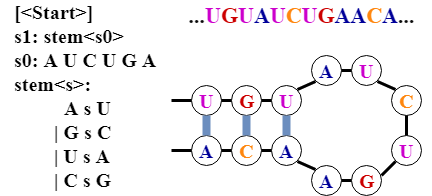
\includegraphics[width=5.5cm]{img4.png}
                \end{center} 
            }
           \end{tabular}
           & \begin{tabular}{l}
           \begin{center}
               
               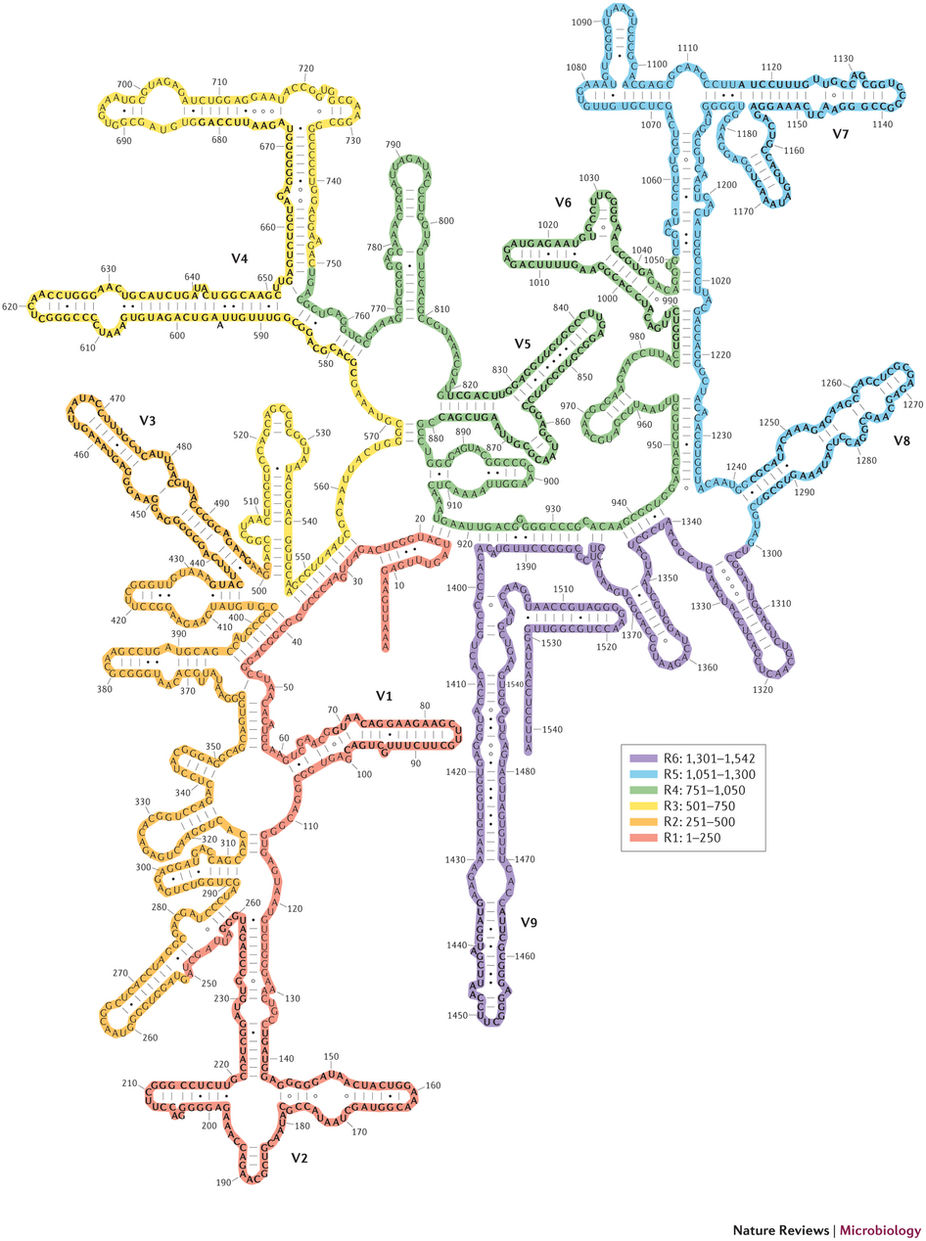
\includegraphics[width=4.5cm,left]{img1.jpg}
                \end{center}
         \end{tabular}  \\
\end{tabular}

           
\end{frame}

\begin{frame}\frametitle{Цель и задачи}
Цель: 

исследование возможности распознавания бактерий на основе данных о вторичной структуре их 16s РНК, полученных методами синтаксического анализа, с помощью машинного обучения.

\vspace{5\onelineskip}

Задачи:
\begin{itemize}
    \item Разработка архитектуры решения
    \item Выбор формата представления данных о вторичной структуре бактерий и реализация процесса их генерации
    \item Создание нейронной сети для распознавания 16s РНК среди прочих нуклеотидных последовательностей
    \item Экспериментальные исследования и анализ полученных результатов
\end{itemize}
\end{frame}

\begin{frame}\frametitle{Похожие решения}

\begin{itemize}
    \item BLAST --- поиск гомологов белков и нуклеиновых кислот на основе их первичной структуры
    \item HMMER --- моделирование вторичной структуры с использованием теории скрытых марковских моделей
    \item Infernal --- моделирование вторичной структуры с помощью вероятностных моделей и стохастических контекстно-свободных грамматик
    \item Humidor --- классификация данных в формате CIGAR strings с помощью сверточных нейронных сетей
\end{itemize}
\end{frame}

\begin{frame}\frametitle{Архитектура решения}
\begin{itemize}
    \item Платформа YaccConstructor
    \item Библиотека Keras
\end{itemize}
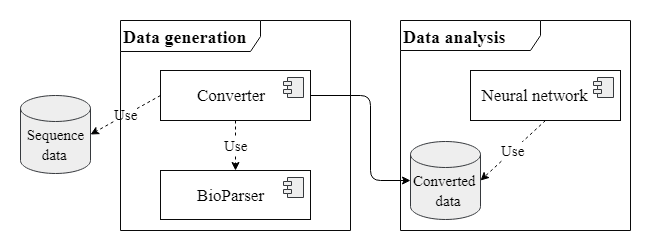
\includegraphics[width=12cm]{architecture.png}
\end{frame}


\begin{frame}\frametitle{Генерация данных}
\begin{itemize}
    \item Имеется последовательность нуклеотидов и некоторая грамматика
    \item С помощью алгоритма синтаксического анализа получается лес разбора, по которому строится матрица
    \item Матрица линеаризуется и преобразовывается в числовой вектор
\end{itemize}
\end{frame}

\begin{frame}\frametitle{Нейронная сеть}

\begin{itemize}
    \item Keras, TensorFlow
    \item Dense и Dropout слои
    \item Данные из БД SILVA
\end{itemize}

\end{frame}

\begin{frame}\frametitle{Эксперименты}
\begin{itemize}
    \item Accuracy = 0.87
    \item Precision = 0.96
    \item Recall = 0.77
    \item Specificity = 0.97
    \item Всего 35706 образцов
    \item 7345 тестовых образцов
\end{itemize}
\vspace{5\onelineskip}
\begin{tabular}{ | l | l | 1 | }
\hline
& classified as positive & classified as negative \\
\hline
positive & 2789 & 856 \\
\hline
negative & 108 & 3592 \\
\hline
\end{tabular}
\vspace{5\onelineskip}
\end{frame}


\begin{frame}\frametitle{Результаты}
\begin{itemize}
    \item Разработана архитектура решения
    \item Реализован процесс генерации данных в виде числовых векторов
    \item Создана нейронная сеть для распознавания 16s РНК бактерий по данным о вторичной структуре
    \item Проведены экспериментальные исследования на участках геномов бактерий из базы данных SILVA
\end{itemize}
\end{frame}
\end{document}